% !TeX program = lualatex
% !TeX encoding = utf8
% !TeX spellcheck = uk_UA
% !TeX root =../MexPractEng.tex

%=========================================================
\chapter{Kinematics}\label{\currfilebase}
\Opensolutionfile{answer}[\currfilebase/\currfilebase-Answers]
\Writetofile{answer}{\protect\section*{\nameref*{\currfilebase}}}%
%=========================================================

\section{Kinematics of the particle}

\subsection{Motion in one dimension}


%=========================================================
\begin{problem}
	An object traveling along the $x$ axis with an initial velocity
	of $5.0$~\si{\meter\per\second} has a constant acceleration of $2.0$~\si{\meter\per\square\second}. When its velocity is $15.0$~\si{\meter\per\second}, how far has it traveled?
\end{problem}


%=========================================================
\begin{problem}
	The position of an object moving along an $x$ axis is given
	by $x = 3t  + 4t^2  + t^3$, where $x$ is in meters and $t$ in seconds. 
	\begin{enumerate}[label = (\alph*)]
		\item Find the position of the object at the following values of $t$: $1$, $2$, $3$ and $4$~s.
		\item Find the velocity of the object at the following values of $t$: $1$, $2$, $3$ and $4$~s.
		\item What is the object's displacement between $t = 0$
		and $t = 4$~s?
		\item \label{av} What is its average velocity for the time interval
		from  $t = 0$~s to  $t = 4$~s?
		\item Graph $x$ versus $t$ for $0 \le x \le 4$ s and indicate how the answer for \ref{av} can be found on the graph.
	\end{enumerate} 
\end{problem}


%=========================================================
\begin{problem}
	The position function $x(t)$ of a particle moving along an $x$ axis
	is $x   = 4.0 + 6.0t^2$, with $x$ in meters and $t$ in seconds.
	\begin{enumerate}[label = (\alph*)]
		\item At what time and where does the particle (momentarily) stop?
		\item At what negative time and positive time does the particle pass
		through the origin?
		\item Graph $x$ versus $t$ for the range $-5$~s to $+5$~s.
		\item To shift the curve rightward on the graph, should we include the
	\end{enumerate}
\end{problem}


%=========================================================
\begin{problem}
	At a certain time a particle had a speed of $18$~m/s in the positive $x$ direction, and $2.4$~s later its speed was $30$~\si{\meter\per\second} in the
	opposite direction.What is the average acceleration of the particle during this $2.4 $~\si{\second} interval?
\end{problem}


%=========================================================
\begin{problem}
	An electric vehicle starts from rest and accelerates at a rate
	of $2.0$~m/s\textsuperscript{2} in a straight line until it reaches a speed of $20$~m/s. The
	vehicle then slows at a constant rate of $1.0$~\si{\meter\per\square\second} until it stops.
	\begin{enumerate}[label = (\alph*)]
		\item How much time elapses from start to stop?
		\item How far does the vehicle travel from start to stop?
	\end{enumerate}
\end{problem}


%=========================================================
\begin{problem}
	A particle moves along the $x$ axis. Its position varies with time according to
	the expression $x =  -4t + 2t^2$, where $x$ is in meters and $t$ is in seconds. 
	\begin{enumerate}[label = (\alph*)]
		\item Graph $x$ versus $t$ for the range $t = 0$~\si{\second} to $t = 4$~\si{\second}.
		\item Determine the displacement of the particle in the time intervals $t = 0$~\si{\second}
		to $t = 1$~\si{\second} and $t = 1$~\si{\second} to $t = 3$~\si{\second}.
		\item Calculate the average velocity during these two time intervals.
		\item Find the instantaneous velocity of the particle at $t = 2.5$~\si{\second}.
	\end{enumerate}
	\begin{solution}
		\begin{enumerate}[label = (\alph*)]
			\item Graph $x$ versus $t$ for the range $t = 0$~\si{\second} to $t = 4$~\si{\second}:		
			
			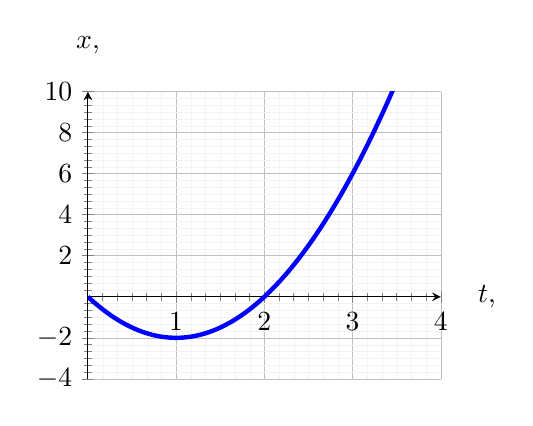
\begin{tikzpicture}
			\begin{axis}[%
			% === Налаштування сітки ===
			grid = both,
			grid style={line width=.1pt, draw=gray!10},
			major grid style={line width=.2pt,draw=gray!50},
			minor tick num = 5,
			minor grid style = {line width=.1pt,draw=gray!10},
			% === Налаштування положення координатних осей ===
			axis lines = middle,
			axis line style={-stealth},
			% === Вибір підписів шкали для відображення ===
			xtick = {0,1,...,4},
			ytick = {-4,-2,...,10},
			% === Підпис координатних осей ===
			xlabel={$t$, \si{\second}},
			ylabel={$x$, \si{\meter}},
			% === Положення підпису координатних осей ===
			xlabel style={right = 10pt},
			ylabel style={above = 10pt},
			% === Налаштування мінімальних та максимальних значень координат ===
			xmin = 0,
			xmax =  4,
			ymin = -4,
			ymax =  10,
			% === Налаштування розміру графіка ===
			width=0.5\linewidth,
			]
			\addplot+[blue, no marks, domain={0:4}, samples=100, ultra thick] {-4*x+2*x^2};
			\end{axis}
			\end{tikzpicture}
			
			\item Displacement of the particle in the time intervals $t = 0$~\si{\second}
			to $t = 1$~\si{\second} is $\Delta x = -2$~\si{\meter},  displacement of the particle in the time intervals $t = 1 $~\si{\second} to $t = 5$~\si{\second} is $\Delta x = + 8$~\si{\meter}.
			\item $\left\langle v\right\rangle  = -2$~\si{\meter\per\second}.
			\item $v_x = 6$~\si{\meter\per\second}.
		\end{enumerate}
	\end{solution}
\end{problem}


%=========================================================
\begin{problem}
	The velocity of a particle moving in the positive direction 
	of the $x$ axis varies as $v = \alpha\sqrt{x}$, where $\alpha$ is a positive constant. 
	Assuming that at the moment $t = 0$ the particle was located at the point $x = 0$, find: 
	\begin{enumerate}[label = (\alph*)]
		\item the time dependence of the velocity and the acceleration of the particle;
		\item the mean velocity of the particle averaged over the time that 
		the particle takes to cover the first s metres of the path.
	\end{enumerate}
	\begin{solution}
		\begin{enumerate*}[label = (\alph*)]
			\item $v = \frac{\alpha t^2}{2}$, $a = \frac{\alpha^2}{2}$;
			\item $\left\langle v \right\rangle = \frac{\sqrt{s}}{2}$.
		\end{enumerate*}
	\end{solution}
\end{problem}


\subsection{Motion in three dimension. The coordinate and vector method}

%=========================================================
\begin{problem}
	An electron's position is given by $\vec r = 3.00t \vec i -4.00 t^2\vec j + 2.00 \vec k$,
	with $t$ in seconds and in meters. 
	\begin{enumerate}[label = (\alph*)]
		\item In unit-vector notation, what is the electron’s velocity $\vec v(t)$? 
		\item At $t = 2.00$~s, what is $\vec v$ in unit-vector,
		\item a magnitude $v$,
		\item an angle relative to 	the positive direction of the $x$ axis?
	\end{enumerate}
\end{problem}


%=========================================================
\begin{problem}
	Aparticle moves in the $xy$ plane with constant acceleration.
	At $t = 0$ the particle is at $\vec r_1 = (4.00~m) \vec i + (3.00~m) \vec j$, with velocity $\vec v_1$.
	At $t = 2.0$~s, the particle has moved to $\vec r_2 = (10.00~m) \vec i + (2.00~m) \vec j$ and
	its velocity has changed to $\vec v_2 = (5.00~m/s) \vec i - (6.00~m/s) \vec j$. 
	\begin{enumerate}[label = (\alph*)]
		\item Find $\vec v_1$.
		\item What is the acceleration of the particle?
		\item What is the velocity of the particle as a function of time?
		\item  What is the position vector of the particle as a function of time?
	\end{enumerate}
\end{problem}


\subsection{Projectile motion}

%=========================================================
\begin{problem}
	A projectile is launched with speed $v_0$ at an angle of $\alpha$
	above the horizontal. Find an expression for the maximum height it
	reaches above its starting point in terms of $v_0$, $\alpha$ and $g$. (Ignore any
	effects due to air resistance.)
\end{problem}


%=========================================================
\begin{problem}
	A projectile is launched from ground level with an initial
	speed of 53~\si{\meter\per\second}. Find the launch angle (the angle the initial velocity vector is above the horizontal) such that the maximum height of
	the projectile is equal to its horizontal range. (Ignore any effects due
	to air resistance.)
\end{problem}


%=========================================================
\begin{problem}
	A ball launched from ground level lands $2.44$~s later on a
	level field $40.0$~m away from the launch point. Find the magnitude
	of the initial velocity vector and the angle it is above the horizontal.
	(Ignore any effects due to air resistance.)
\end{problem}


%=========================================================
\begin{problem}
	At $\nfrac12$ of its maximum height, the speed of a projectile is $\nfrac34$
	of its initial speed. What was its launch angle? (Ignore any effects
	due to air resistance.)
	\begin{solution}
		$\alpha =69.3^\circ$.
	\end{solution}
\end{problem}


%=========================================================
\begin{problem}\label{prb:kin_ball_to_wall}
	A ball is to be shot from level ground toward a wall at distance $x$ (Fig.~\ref{kin_ball_to_wall_pic}). Figure~\ref{kin_ball_to_wall_plot} shows the $y$ component $v_y$ of the ball’s velocity just as it would reach the wall, as a function of that distance $x$. What is the launch angle?
%=========================================================
\begin{figure}[h!]\centering
	%---------------------------------------------------------
	\begin{subfigure}[t]{0.45\linewidth}\centering
		\begin{tikzpicture}
			\node (ground) [ground,anchor=north,yshift=-0.2cm,minimum width=5cm,xshift=2.03cm] {};
			\draw (ground.north east) -- (ground.north west);
			
			\node (fill) [ground,xshift=-0.15cm,minimum height = 0.3cm, minimum width = 0.3cm] at (ground.west) {};
			
			\node (wall) [ground, rotate=-90, minimum width=4cm,anchor=south east] at (fill.north west) {};
			\draw (wall.north east) -- (wall.north west);
			
			\draw[-latex] (4,0) -- +(0,4) node[above] {$y$};
			\draw[-latex] (4,0) -- +(-5,0) node[above] {$x$};
			\draw[ultra thick, -latex] (4,0) -- +(135:2) node[above] {$\vec v$};
			\draw[ball color = red] (4,0) circle(0.3);
			\draw (4,0) +(180:0.5) arc (180:135:0.5) node[left, pos=0.5] {$\alpha$};
		\end{tikzpicture}
		\caption{}
		\label{kin_ball_to_wall_pic}
	\end{subfigure}
	%---------------------------------------------------------
	\begin{subfigure}[t]{0.45\linewidth}\centering
		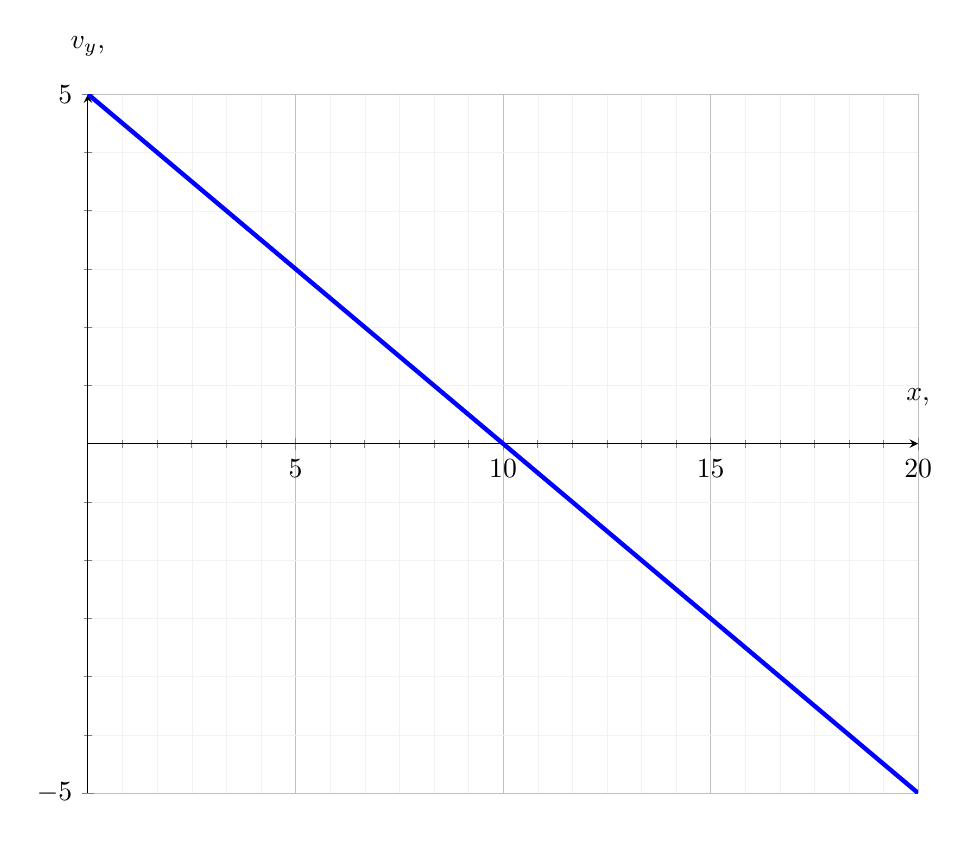
\begin{tikzpicture}
			\begin{axis}[%
			% === Налаштування сітки ===
			grid = both,
			grid style={line width=.1pt, draw=gray!10},
			major grid style={line width=.2pt,draw=gray!50},
			minor tick num = 5,
			minor grid style = {line width=.1pt,draw=gray!10},
			% === Налаштування положення координатних осей ===
			axis lines = middle,
			axis line style={-stealth},
			% === Вибір підписів шкали для відображення ===
			xtick = {0,5,...,20},
			ytick = {-5,0,5},
			% === Підпис координатних осей ===
			xlabel={$x$, \si{\meter}},
			ylabel={$v_y$, \si{\meter\per\second}},
			% === Положення підпису координатних осей ===
			xlabel style={above = 10pt},
			ylabel style={above = 10pt},
			% === Налаштування мінімальних та максимальних значень координат ===
			xmin = 0,
			xmax =  20,
			ymin = -5,
			ymax =  5,
			% === Налаштування розміру графіка ===
			width=\linewidth,
			]
			\addplot+[blue, no marks, domain={0:20}, samples=100, ultra thick] {5-0.5*x};
			\end{axis}
		\end{tikzpicture}
		\caption{}
		\label{kin_ball_to_wall_plot}
	\end{subfigure}
	%---------------------------------------------------------
	\caption{Problem~\ref{prb:kin_ball_to_wall}}
\end{figure}
%=========================================================
\end{problem}



\subsection{Circular motion. Natural description of the motion}

%=========================================================
\begin{problem}
	A point moves along a circle with a velocity $v = \alpha t$, where $a = 0.50$~m/s\textsuperscript{2}. Find the total acceleration of the point at the moment when it covered the $n = 0.10$ fraction of the circle after the beginning of motion. 
	\begin{solution}
		$a = \alpha\sqrt{1 + (4\pi n)^2}$~0.8~m/s\textsuperscript{2}.
	\end{solution}
\end{problem}

%=========================================================
\begin{problem}
	What is the angular speed of Earth in radians per second as it rotates about its axis?
\end{problem}

%=========================================================
\begin{problem}
	A point moves in the plane so that its tangential acceleration 
	$a_\tau = \alpha$, and its normal acceleration $a_n = \beta t^4$, where $\alpha$ and $\beta$ are positive constants, and $t$ is time. At the moment $t = 0$ the point was 
	at rest. Find how the curvature radius $R$ of the point's trajectory and 
	the total acceleration $a$ depend on the distance covered $s$. 
	\begin{solution}
		$R = \frac{\alpha^3}{2\beta s}$, $a = \alpha\sqrt{1 + \left(\sqrt{\frac{4\beta s^2}{\alpha^3}} \right) }$.
	\end{solution}
\end{problem}

%=========================================================
\begin{problem}
	A point moves in the plane $xy$ according to the law $x = A\sin\omega t$, $y = A (1 - \cos\omega t)$, where $A$ and $\omega$ are positive constants. Find:
		\begin{enumerate}[label = (\alph*)]
			\item the distance $s$ traversed by the point during the time $\tau$; 
			\item the angle between the point's velocity and acceleration vectors.
		\end{enumerate}		
	\begin{solution}
		\begin{enumerate*}[label = (\alph*)]
			\item $s = A\omega \tau$, 
			\item $\nfrac{\pi}{2}$.
		\end{enumerate*}
	\end{solution}
\end{problem}


%=========================================================
\begin{problem}
	A point moves along an arc of a circle of radius $R$. Its velocity 
	depends on the distance covered $s$ as $v = \alpha\sqrt{s}$, where $\alpha$ is a constant. 
	Find the angle a between the vector of the total acceleration and 
	the vector of velocity as a function of $s$. 
	\begin{solution}
		$\tan\alpha = \frac{2s}{R}$
	\end{solution}
\end{problem}

\section{Rotational motion and its angular characteristics. Kinematics of a rigid body}


%=========================================================
\begin{problem}
	What is the angular speed of 
	\begin{enumerate*}[label = (\alph*)]
		\item the second hand,
		\item the minute hand,
		\item and the hour hand
	\end{enumerate*}	
of a smoothly running analog watch? Answer in radians per second.
\end{problem}


%=========================================================
\begin{problem}
	The angular position of a point on a rotating wheel is given
	by $\phi = 2.0 + 4.0t^2 + 2.0t^3$, where $\phi$ is in radians and $t$ is in seconds. At
	$t = 0$, what are 
	\begin{enumerate*}[label = (\alph*)]
		\item the point’s angular position
		\item and its angular velocity?
		\item What is its angular velocity at $t = 4.0$~s?
		\item Calculate its angular acceleration at $t = 2.0$~s.
		\item Is its angular acceleration constant?
	\end{enumerate*}
\end{problem}


%=========================================================
\begin{problem}
	The angular position of a point on the rim of a rotating wheel is
	given by $\phi = 4.0t - 3.0t^2 + t^3$, where $\phi$ is in radians and $t$ is in seconds.
	What are the angular velocities at 
	\begin{enumerate*}[label = (\alph*)]
		\item $t = 2.0$~s
		\item and $t = 4.0$~s?
		\item What is the average angular acceleration for the time interval that begins at $t = 2.0$~s and ends at $t = 4.0$~s?
		What are the instantaneous angular accelerations at
		\item the beginning
		\item and the end of this time interval?
	\end{enumerate*}
\end{problem}


%=========================================================
\begin{problem}
	A $12$-cm-radius disk that begins to rotate about its axis at $t = 0$,
	rotates with a constant angular acceleration of $8.0$~\si{\radian\per\square\second}. At $t = 5$~\si{\second} find:
	\begin{enumerate}[label = (\alph*)]
		\item what is the angular speed of the disk,
		\item  what are
		the tangential and centripetal components of the acceleration of a
		point on the edge of the disk?
	\end{enumerate}
\end{problem}


%=========================================================
\begin{problem}
	A solid body rotates with angular velocity $\vec \omega = a t\vec i + b t^2 \vec j$, 
	where $a = 0.50$~\si{\radian\per\square\second}, $b = 0.060$~\si{\radian\per\cubic\second}. Find:
	\begin{enumerate}[label = (\alph*)]
		\item the magnitude of the angular velocity and the angular acceleration 
		at the moment $t = 10.0$~s;
		\item the angle between the vectors of the angular velocity and the 
		angular acceleration at that moment. 
	\end{enumerate} 
	\begin{solution}
		\begin{enumerate*}[label = (\alph*)]
		\item $\omega = 8.0$~\si{\radian\per\second}, $\beta = 1.3$~\si{\radian\per\square\second};
		\item $17^\circ$.
		\end{enumerate*}	
	\end{solution}
\end{problem}


%=========================================================
\begin{problem}
	A solid body rotates about a stationary axis so that its angular velocity depends on the rotation angle $\omega = \omega_0 - a\phi$, where 
	$\omega_0$ and $a$ are positive constants. At the moment $t = 0$ the angle 
	$\phi = 0$. Find the time dependence of
	\begin{enumerate*}[label = (\alph*)]
	 	\item the rotation angle; 
	 	\item the angular velocity.
	\end{enumerate*}
	\begin{solution}
		\begin{enumerate*}[label = (\alph*)]
			\item $\phi = \frac{\omega_0}{a}(1- e^{-at})$; 
			\item $\omega = \omega_0e^{-at}$.
		\end{enumerate*}
	\end{solution}
\end{problem}


\Closesolutionfile{answer}

